% This is "sig-alternate.tex" V2.1 April 2013
% This file should be compiled with V2.5 of "sig-alternate.cls" May 2012
%
% This example file demonstrates the use of the 'sig-alternate.cls'
% V2.5 LaTeX2e document class file. It is for those submitting
% articles to ACM Conference Proceedings WHO DO NOT WISH TO
% STRICTLY ADHERE TO THE SIGS (PUBS-BOARD-ENDORSED) STYLE.
% The 'sig-alternate.cls' file will produce a similar-looking,
% albeit, 'tighter' paper resulting in, invariably, fewer pages.
%
% ----------------------------------------------------------------------------------------------------------------
% This .tex file (and associated .cls V2.5) produces:
%       1) The Permission Statement
%       2) The Conference (location) Info information
%       3) The Copyright Line with ACM data
%       4) NO page numbers
%
% as against the acm_proc_article-sp.cls file which
% DOES NOT produce 1) thru' 3) above.
%
% Using 'sig-alternate.cls' you have control, however, from within
% the source .tex file, over both the CopyrightYear
% (defaulted to 200X) and the ACM Copyright Data
% (defaulted to X-XXXXX-XX-X/XX/XX).
% e.g.
% \CopyrightYear{2007} will cause 2007 to appear in the copyright line.
% \crdata{0-12345-67-8/90/12} will cause 0-12345-67-8/90/12 to appear in the copyright line.
%
% ---------------------------------------------------------------------------------------------------------------
% This .tex source is an example which *does* use
% the .bib file (from which the .bbl file % is produced).
% REMEMBER HOWEVER: After having produced the .bbl file,
% and prior to final submission, you *NEED* to 'insert'
% your .bbl file into your source .tex file so as to provide
% ONE 'self-contained' source file.
%
% ================= IF YOU HAVE QUESTIONS =======================
% Questions regarding the SIGS styles, SIGS policies and
% procedures, Conferences etc. should be sent to
% Adrienne Griscti (griscti@acm.org)
%
% Technical questions _only_ to
% Gerald Murray (murray@hq.acm.org)
% ===============================================================
%
% For tracking purposes - this is V2.0 - May 2012

\documentclass{sig-alternate-05-2015}
\usepackage{lipsum}% http://ctan.org/pkg/lipsum
\usepackage{graphicx}% http://ctan.org/pkg/graphicx
\usepackage{float}
\usepackage{todonotes}
\usepackage{color}
\usepackage[outdir=./figures/]{epstopdf}
\usepackage{listings}
\begin{document}
%\lstset{numbers=left, numberstyle=\small, numbersep=8pt, frame = single, language=Pascal, framexleftmargin=15pt}


% Copyright
\setcopyright{acmcopyright}
%\setcopyright{acmlicensed}
%\setcopyright{rightsretained}
%\setcopyright{usgov}
%\setcopyright{usgovmixed}
%\setcopyright{cagov}
%\setcopyright{cagovmixed}


% DOI
%\doi{10.475/123_4}

% ISBN
%\isbn{123-4567-24-567/08/06}

%Conference
\conferenceinfo{SIGMOD '17}{May 14--19, 2017, Raleigh, North Carolina, USA}

%\acmPrice{\$15.00}

%
% --- Author Metadata here ---
%\conferenceinfo{WOODSTOCK}{'97 El Paso, Texas USA}
%\CopyrightYear{2007} % Allows default copyright year (20XX) to be over-ridden - IF NEED BE.
%\crdata{0-12345-67-8/90/01}  % Allows default copyright data (0-89791-88-6/97/05) to be over-ridden - IF NEED BE.
% --- End of Author Metadata ---

\title{A Novel Approach to Continuous Training of Large Scale Machine Learning Models}

%
% You need the command \numberofauthors to handle the 'placement
% and alignment' of the authors beneath the title.
%
% For aesthetic reasons, we recommend 'three authors at a time'
% i.e. three 'name/affiliation blocks' be placed beneath the title.
%
% NOTE: You are NOT restricted in how many 'rows' of
% "name/affiliations" may appear. We just ask that you restrict
% the number of 'columns' to three.
%
% Because of the available 'opening page real-estate'
% we ask you to refrain from putting more than six authors
% (two rows with three columns) beneath the article title.
% More than six makes the first-page appear very cluttered indeed.
%
% Use the \alignauthor commands to handle the names
% and affiliations for an 'aesthetic maximum' of six authors.
% Add names, affiliations, addresses for
% the seventh etc. author(s) as the argument for the
% \additionalauthors command.
% These 'additional authors' will be output/set for you
% without further effort on your part as the last section in
% the body of your article BEFORE References or any Appendices.

\numberofauthors{4} %  in this sample file, there are a *total*
% of EIGHT authors. SIX appear on the 'first-page' (for formatting
% reasons) and the remaining two appear in the \additionalauthors section.
%
\author{
% You can go ahead and credit any number of authors here,
% e.g. one 'row of three' or two rows (consisting of one row of three
% and a second row of one, two or three).
%
% The command \alignauthor (no curly braces needed) should
% precede each author name, affiliation/snail-mail address and
% e-mail address. Additionally, tag each line of
% affiliation/address with \affaddr, and tag the
% e-mail address with \email.
%
% 1st. author
\alignauthor
Author 1
% 2nd. author
\alignauthor
Author 2
% 3rd. author
\alignauthor Author 3
\and  % use '\and' if you need 'another row' of author names
% 4th. author
\alignauthor Author 4
}

\maketitle

\begin{abstract}
Machine learning is increasingly pervasive in many business and scientific applications. 
Making machine learning models ready for serving in a productive environment is a process done in form of pipelines that include several manual, semiautomatic, and automatic steps. 
Model deployment is the final stage in these pipelines.
Once a machine learning model is trained on an initial dataset it is deployed into a system where it can answer prediction queries in a realtime and reliable fashion.
If new training data becomes available while the system is running, the model is updated.
Currently, these updates are either performed incrementally (one at a time) or they require a complete retraining of the model offline.

In this paper, we propose a novel deployment method for stochastic gradient descent (SGD)-based machine learning models.
SGD is an iterative process, which works well with large data sets.
In each iteration of SGD, the model is updated based on one or a sample (mini-batch) of the training items.
Using this property of SGD, not only incremental learning can be applied but we also eliminate the need for offline retraining and replace it with continuous mini-batch updates.
One iteration of SGD is lightweight and can be executed while the system is running without interrupting the normal flow.
Our experiments show that our deployment method can achieve up to an order of magnitude faster model update without degrading the quality of the model and in some case even increasing the quality due to faster adoption to changes in data distribution.


\end{abstract}


%
% The code below should be generated by the tool at
% http://dl.acm.org/ccs.cfm
% Please copy and paste the code instead of the example below. 
%


%
% End generated code
%

%
%  Use this command to print the description
%
%\printccsdesc


\keywords{ML Model Management; Stochastic Gradient Descent; ML Systems}

\section{Introduction}
% Problem
Deployment and maintenance of machine learning models is a crucial step in machine learning applications' life cycle. 
However, it is one that has received very little attention. 
% Why is it important
ML application's life cycle does not end with training. 
In fact deployment and serving of the models is the most crucial part that brings the actual business value. 
% Specific problem
In order to gain actual value out of a machine learning model, it has to be monitored in realtime in production environment. 
These models have to be maintained and constantly updated incrementally to better fit the new data that arrives. 
The models should also be deployed in an environment that is capable of handling high traffic. 
While all of these are happening, the models should be re-trained since ML models usually need to have access to entire datasets, otherwise the quality will degrade if they are only updated incrementally.
% How is it different from prior work
Most of the machine learning systems focus on training and providing tools to make model training and search easier. 
Kumar et al. \cite{kumar2015survey} provided an overview of landscape of existing machine learning systems. 
Except in a very few cases \cite{akdere2011case, crankshaw2014missing}, most of the surveyed systems, focus on training of machine learning models and provide little to no support after the model has been trained.
Moreover, systems with support for model deployment are still lacking constant monitoring and fast and accurate updates of the machine learning models.
% What is the motivation for this work
Given the lack of systems to support model deployment and maintenance we have set out to design a system that not only support deployment and maintenance of machine learning models but also provide constants incremental and batch updates while the system is running. 
We propose the design of a system that provide realtime query support as well incremental and fast batch updates to the machine learning models.

\subsection{Model management and serving} \label{model-management-serving}

\todo[inline]{this reads more like related work. You can make it background, then it should be before or after SGD.}

\begin{figure*}[t]
\centering
\includegraphics[scale = 0.4]{../images/current-method.png}
\caption{Velox Work Flow}
\label{fig:velox-work-flow}
\end{figure*}

Traditional machine learning systems focus on training and management of models and leave the task of deployment and maintenance to the users. 
It has only been recently that some systems, for example Velox \cite{crankshaw2014missing}, TensorFlow Serving \cite{abadi2016tensorflow}, and LongView \cite{akdere2011case} have proposed architectures to support model deployment and query answering as well. 
LongView integrates predictive machine learning models into relational databases. 
It answers predictive queries and maintains and manages the models.
LongView uses techniques such as query optimization and materialized view selection to increase the performance of the system.
TensorFlow Serving provides mechanisms for realtime queries, deployment and version control of machine learning models.
It has out-of-the-box support for models created using TensorFlow and it provides several interfaces for users to deploy their custom models.
However, it does not provide incremental updates to the model.
Models have to be recreated outside of the system by the user and redeployed into TensorFlow Serving.
Similarly, Velox provides a set of interfaces for users to deploy their models. 
It is integrated into the \textit{Berkeley Data Analytics Stack (BDAS)}, and uses the components of BDAS such as Tachyon \cite{li2014tachyon} and Spark \cite{zaharia2010spark}. 
Models are typically trained offline using Spark. 
Once a model is trained, it is deployed using Velox and Velox can answer prediction queries in realtime and perform incremental updates to the model.
Velox also monitors the quality of the model using a validation set and once the error rate has gone beyond a predefined threshold it initiates a complete retraining of the model using Spark. 
Figure \ref{fig:velox-work-flow} depicts how Velox works. 
While all of these systems provide intuitive mechanisms for model deployment, they have some drawbacks. 
LongView only works with static data and does not have support for realtime queries.
TensorFlow Serving completely separates the process of model training from model serving. 
It requires the users to train the model separately and while the model is being served, it does not perform incremental updates to the model.
Velox has addressed these problems. 
It provides a mechanism for realtime query support as well as incremental updates to the model.
It allows retraining of the models offline when the quality has fallen bellow a predefined threshold.
Velox provides an API that when called will initiate an out-of-core offline retraining of the model.
It uses Stochastic Gradient Descent (SGD) optimization to train the models offline in Apache Spark.
This batch process affects the system and heavily slows down the model update process.

% What are the contributions
\subsection{Contributions and paper outline}
\todo[inline]{this should be part of the intro}
Our key observation is that, by utilizing the underlying optimization algorithm (SGD), the model training process can be seamlessly executed along side the serving and query answering component.
Based on this observation, we present a new model for a system, that supports deployment, maintenance, and incremental and fast batch updates of machine learning models.
We are making the following contributions: 
\begin{itemize}
\item a system for machine learning models deployment and maintenance
\item uninterrupted batch updates to the model while the system is running
\item incremental updates and handling of changes in data distribution (concept drift) 
\end{itemize}
% What are the main results
Our experiments show that we are able to achieve the same quality with similar systems while completely eliminating the offline batch training, which reduces the running time by an order of magnitude. 
We have experimented on time dependent datasets where distribution of the data changes over time and we have shown that our method can adapt to changes in the distribution.
% Outline: The rest of this document is structured as follows. ...
The rest of this paper is organized as follows. 
Section \ref{sgd} describes the underlying optimization method used in our system. 
Section \ref{continious-training-serving} discusses the architecture and details of our system. 
In section \ref{tuning}, we explore the different parameters of the system and how the automatic tuning of these parameters further improve the performance.
Section \ref{evaluation} compares the performance of our system with similar model serving and management systems. 
Related work is discussed in section \ref{related-work} and in section \ref{conclusion} we conclude our 


\section{Stochastic Gradient Descent} \label{sgd}
In machine learning, optimization methods are used to find the minimum of the objective function (referred to as the loss function) by calculating the gradient of the function at different data points and update the function parameters based on the gradient values.
A common optimization method is gradient descent, an iterative process where in every iteration the entire training data set is used to calculate the gradient value.
One drawback of gradient descent is that in presence of large datasets it will become very slow since every iteration has to inspect all the training items.
stochastic gradient descent (SGD) is an approximation of the gradient descent method. 
Similar to gradient descent, it is an iterative process but in each iteration it operates on one element (or a sample of elements) at a time. 
It calculates the gradient at a single element and updates the parameters of the model accordingly. 
Although it converges after a higher number of iterations, the overall convergence time is still much faster than gradient descent. 
Each iteration of SGD can be executed in a short amount of time since it only works with a sample of the data.
We are leveraging this property of SGD and design the system so that it executes one iteration of SGD at a time while the system is running.
In our experiments, \todo[inline]{maybe reference section} we show that time to execute single iteration of SGD is insignificant.
Moreover, since a single iteration is a lightweight process, it can be executed in separate threads. \todo[inline]{that does not make sense to me, is it independent? then it can be executed in separate threads}

\subsection{Distributed SGD}
{\color{red} should I even include this section? - I would TR}
\todo[inline]{this needs to be expanded to explain why parallelization and distribution might be desirable}
One problem in distributed environment is synchronizing the updates from different nodes. 
It has slowed down the SGD process, because after every iteration, all the updates are sent to a master node that updates the model.
\cite{recht2011hogwild, dean2012large} proposed distributed asynchronous SGD and the experimental results showed that the quality of the final model is not any worse than the synchronized approach. 


\subsection{Learning rate tuning} \label{learning-rate}
The learning rate or step size parameter plays an important role in the convergence of SGD.
The most common technique is to set the learning rate to a small value, and slowly decrease the value in every iteration. 
This, however is not possible in case of continuous and online learning. 
Adaptive learning rates have been used in online scenarios where based on different criteria the learning rate is adjusted automatically.
Schaul et al. \cite{schaul2013no} have proposed one such method were the learning rate can be inferred automatically based on the changes in the weight parameters. 
One advantage of their method is that it works well with non-stationary problems, where the distribution of the data is constantly changing. 
By examining the changes in the data the learning rate will decrease (when approaching the optimum value) and increase (when the distribution of the data has changed).
 
{\color{red}Not yet implemented - either you have some more info about thresholds etc. or you have to leave this out.}
We use this strategy in our implementation of SGD. 


\subsection{Machine learning models based on SGD}
SGD is one of the most common optimization methods to train large scale problems. 
It has been used in classification \cite{zhang2004solving}, clustering \cite{bottou1995convergence}, neural networks \cite{dean2012large}, and matrix factorization \cite{funk2006netflix}.
In our system, we implemented matrix factorization and neural networks, which will be explained next. 

\textbf{Matrix Factorization} is a common method used in recommender systems \cite{koren2009matrix}. 
Matrix factorization is used to derive the latent factors (users and items) for recommender systems.
It relies on the fact that each user and item can be described in a few dimensions (10 to 40 usually) based on the available ratings.
These latent factors have automatically capture the similarity of users and items based on the ratings provided by the users.
Any unknown rating, hence can be predicted by simply using a dot product of the user vector with item vector.
We used the SGD implementation of matrix factorization by Simon Funk \cite{funk2006netflix}. 
A scalable version of the algorithm was proposed by Gemulla et al. \cite{gemulla2011large}.

\textbf{Neural Networks} or deep learning inspired by biological neural networks in brain are used to learn and approximate complex functions. 
They have been used for more than half a century to model functions and have been used in training machine learning models.
However, due to slow training process and lack of large amount of training data they have not been extensively in machine learning community.
Past decade saw a change with publication of several nominal works.
Hinton et al. \cite{hinton2006fast} proposed methods for speeding up the training of neural networks.
ImageNet competition \cite{ILSVRC15} in 2012 was won by a neural networks approach proposed by Krizhevsky et al. \cite{krizhevsky2012imagenet} where they significantly reduced the error rate. 
Success of Google Brain team \cite{sutskever2014sequence, mikolov2013efficient} was also instrumental to popularizing neural networks in machine learning community.
We have implemented a multilayer neural network for classifying images. {\color{red}explain more?}

\section{Continuous Training and Serving} \label{continious-training-serving}

\begin{figure}[h]
\centering

\includegraphics[scale=0.30]{../images/placeholder.jpeg}
\caption{System Architecture}
\label{fig:system-architecture}
\end{figure}

\begin{figure*}[h]
\centering
\includegraphics[scale=0.45]{../images/continuous.png}
\caption{Continuous Training and Serving}
\label{fig:cont-training-serving}
\end{figure*}

% Stochastic Gradient System properties
As described in Section \ref{sgd}, stochastic gradient descent is an iterative process where in each iteration one or a sample of the data is selected randomly and the gradient is calculated based on this sample. 
After each iteration the parameters of the model are updated.
This means that at the end of an iteration, the model can be used to make predictions.
As more iterations are executed, the model becomes more and more accurate.
This property of stochastic gradient descent makes it ideal for long running systems where prediction requests are arriving at the system continuously.
% We take advantage of the underlying optimization method and design the system around it
% We take advantage of these properties of SGD.
% We do not need complete re-training, each iteration of SGD is light and can be easily executed while the system is running
Since each iteration of SGD is light and fast, it can be done while the system is serving prediction requests.
% figure
Figure \ref{fig:cont-training-serving} shows the details of our proposed system.
An initial model is trained using the data residing on disk.
Once the model is deployed, it receives prediction queries and training observations in a streaming fashion.
Incoming prediction queries are answered as soon as they are received.
Once a training observation is received the model's incremental update method is called and the training item is passed to this method.
The system also keeps track of incoming training observations and adds them to an intermediate buffer.
A scheduler component, will schedule a new iteration of SGD based on the rate of incoming training observations. 
The scheduler can also decide to run an iteration if the system is idle or the load on the system is not heavy. 
Each new iteration will use a random sample of the data in storage and the data in the buffer. 
As more training observations becomes available the model is updated further.
Figure \ref{fig:system-architecture} shows the overview of the architecture of our system.
Next, we explain each part of the system in more detail.

\subsection{Scheduler}\label{scheduler}
Scheduler component is responsible for scheduling of new iterations of SGD.
An iteration of SGD can be scheduled at any point in time.
Intuitively, the best time to execute an iteration is when the system is not under heavy load.
This will help in utilizing the system's resources as well as keeping the model up to date at all time.
Another situation that a new iteration of SGD should be executed is when the system is receiving a lot of training items and the intermediate buffer is getting full.
If the model is not updated with the new training items frequently, the quality will go down more rapidly, especially if the distribution of the data is changing rapidly.
Incremental updates are turned off when a new iteration is scheduled to execute.
Training iterations and model serving are disjoint and not affected by each other.
As soon as the training iteration is completed the model is updated and incremental update is reenabled. \todo[inline]{have you described incremental update vs iterations already? Maybe this could go into background as well}
This property allows the scheduler to execute new iteration of SGD in a separate thread without interrupting the serving module.
The scheduling rate however affects the quality of the model.
Each new iteration slightly increases the quality of the model.
The increase in quality is even more when new training observations have arrived at the system.
In Section \ref{evaluation}, we investigate the effect of scheduling rate on model quality.
In case no new training data is available, the model parameters will converge after awhile and any further training iterations will not have any effect on the model quality.
Therefore, the scheduler component has to communicate with the model manager in order to detect whether the model parameters have converged and stop further iterations until more training data becomes available.

%Tilmann needs to continue here...

\subsection{Data Manager} \label{data-manager}
In order to execute an iteration of SGD, we need to combine the training data that arrives at the system in realtime and the data stored on disk.
Data manager is responsible for storing the incoming training observations in an intermediate buffer.
When a new training iteration is scheduled, data manager accesses the historical data stored on disk and provides a sample based on the configured sampling rate.
The data from the sample and the data in the buffer are merged together to create the dataset for next training iteration.
Data manager provides access to this dataset for model manager where the actual training and model updates happen.
The data manager also communicates with scheduler in order to inform it when the intermediate buffer is becoming full and a new training iteration is required. 

The created data set as described earlier, consists of the data inside the buffer and a sample of the historical data.
The sampling rate therefore is a parameter that has to be configured.
It can be pre-configured to a constant value based on the application.
However, using the feedback from the system's model manager (section \ref{model-manager}), sampling rate can be adjusted.
For example, when data distribution is changing more rapidly smaller sampling rate will put more emphasis on the data that arrived in the system recently. 
This is similar to the problem of concept drift, where the distribution of the incoming data changes overtime.
This will render historical data less important, and as a result a smaller sample of the historical data (or none at all) will give more importance to the data in the buffer and help the model to adopt faster to the concept drift.
However, if there is no concept drift in the data, larger sampling rate will increase the quality of the model after a training iteration.
Another effect that sampling rate has on the system is the training iteration running time.
Larger sampling rate increases the running time of each training iteration as more data has to be processed.
In section \ref{evaluation}, we investigate the effects of different sampling rate on both the quality and performance of the system.

\subsection{Model Manager} \label{model-manager} 
An important part of the system is model manager component.
It is responsible for storing the model, answering prediction queries and performing incremental and batch updates to the model.
Listing \ref{model-manager-api} shows the APIs of model manager.
They are used to both interact with other components as well as end-users of the system.
Scheduler component uses \textit{update} and \textit{update\_batch} to instruct the model manager to perform incremental or batch updates to the model.
Upon a new prediction query, the \textit{predict} method is called to provide the end-user with the label of the given input.
\begin{lstlisting}[language=Scala, basicstyle=\small\ttfamily, frame=tb ,columns=fullflexible,
showstringspaces=false,label=model-manager-api,caption=Model Manager API, numberstyle=\tiny]
def update(x,y)

def update_batch(X,Y)

def predict(x): Label

def error_rate(X_test, Y_test): Double

\end{lstlisting}
\textit{error\_rate} method returns the mean squared error rate of the model using the provided test dataset.
As described earlier, constant monitoring of the quality is required in order to adjust the scheduling and sampling rate.
When the error rate is stagnating, this could mean that the model has converged using the existing data therefore model manager informs scheduler not to schedule any new iterations until new training observations have arrived at the system.
Similarly as explained in section \ref{data-manager}, an increase in error rate could indicate a change in distribution of the data.
As a result, reducing the sampling rate will put more emphasis on the recent data (in the intermediate buffer) and help adopt the model to the changes in the distribution.

Model manager also keeps track of the changes that are made to the model.
The model is updated both through incremental learning and training iteration.
Model manager, creates snapshots of the model in two different scenarios; after a series incremental updates are made and after each training iteration.
This versioning of the models is essential.
When there is a rapid change in the distribution of the incoming data (a sudden concept drift) or when there are anomalies in the data, it is sometimes necessary to revert back to a version before the change in distribution occurred.
In case of concept drift, new training iterations should be scheduled that only use the data in the buffer and in case of an anomalies in the data, they have to be identified and discarded before any further model updates could happen.

\subsection{Distributed environment} 
% How would it scale
As described earlier the underlying optimization method is SGD.
Any computation model capable of executing SGD efficiently can be used as the run-time of the system.
All of the components of the system described so far are not limited to any computation environment.
However, in order to ensure scalability several considerations have to made with regards to each component.
Data manager should be able to work on top of distributed file systems such HDFS \cite{shvachko2010hadoop}. 
In order to allow fast processing of incoming training observations, the intermediate buffer should be stored in memory.
Therefore, the buffer has to be distributed to all the nodes in the computing cluster.
Certain type of machine learning models may be too large to fit into one single node.
One example of such models is the matrix factorization model for recommender systems.
Model manager should partition the model among all the nodes.
It is important that model chose the partitioning strategy in such a way, that when requested the predictions can be made quickly.
For example, when a prediction request for a specific user and item arrives at the system, the model manager should be able to quickly find the related user and item from the matrices to quickly compute the predicted rating for the specific pair.
Our model serving ystem is also not limited to any specific run-time and can accomodate any of the common data processing engines.
Apache Flink \cite{carbone2015apache, alexandrov2014stratosphere} and Apache Spark \cite{zaharia2010spark} are distributed data processing platform that work with data in memory and they have support for iterative algorithms.


\section{Evaluation} \label{evaluation} 
% One more dataset (classification)
% more explanation of the results
% one more experiment (only train on initial data)
In this section, we evaluate the performance of our system using various datasets. 
We report both the quality (error rate) and running time of the system. 
We compare the performance of our system with Velox \cite{crankshaw2014missing}, a purely incremental approach and a fully batch approach where for every new training item that arrives at the system a new model is trained from scratch.

\subsection{Experimental setup}
We run our experiments on a single node with Quad core Intel i7 and 16 GB of RAM. 

\subsection{Datasets}
\textbf{MovieLens \cite{harper2016movielens}}: to analyze the performance of our method on time varying datasets, we use the MovieLens 100K and 1M datasets. 
They consists of movie ratings by users during different time periods. 
For both of the datasets, we use 10\% for initial learning (9\% training, 1\% test) and 90\% for online learning. 
We have set the learning rate to 0.001 for all of the experiments on MovieLens dataset.

\textbf{CIFAR-10 \cite{krizhevsky2009learning}}: this dataset consists of 60000 32x32 color images in 10 classes, with 6000 images per class. We use a Neural Network to train a model to classify the images in the data set. Similar to MovieLens, 10\% are used for initial training and 90\% for online learning. Note that, in this dataset, the order is irrelevant and we assume no change in distribution of the data occurs throughout the system's lifetime. 

\subsection{Tuning parameters} \label{tuning}
In section \ref{continious-training-serving}, we discussed how system parameters such as sampling and scheduling rate affect the performance and quality of the system.
In this section, we are analyzing the effects of different values sampling and scheduling rate on the system.
We 
Our goal, is to make these parameters adaptive, but for now we analyze their effect on the running time and mean squared error. 

\textbf{Scheduling rate}\\
This parameter specifies how often a new iteration of SGD should be scheduled. 
In our prototype the scheduling rate is governed by a parameter called \textbf{Buffer Size}, which dictates how many new items should be stored in the buffer before a new iteration of SGD is executed. 
Ultimately, the decision to schedule new iterations will be made by the system based on the availability of resources. 
Executing one iteration of SGD even using the entire data is not a resource heavy process, and can easily be done in parallel with the serving component of the system. 
This results in a paradigm where both training and serving can happen simultaneously. 

\begin{figure}[H]
\centering
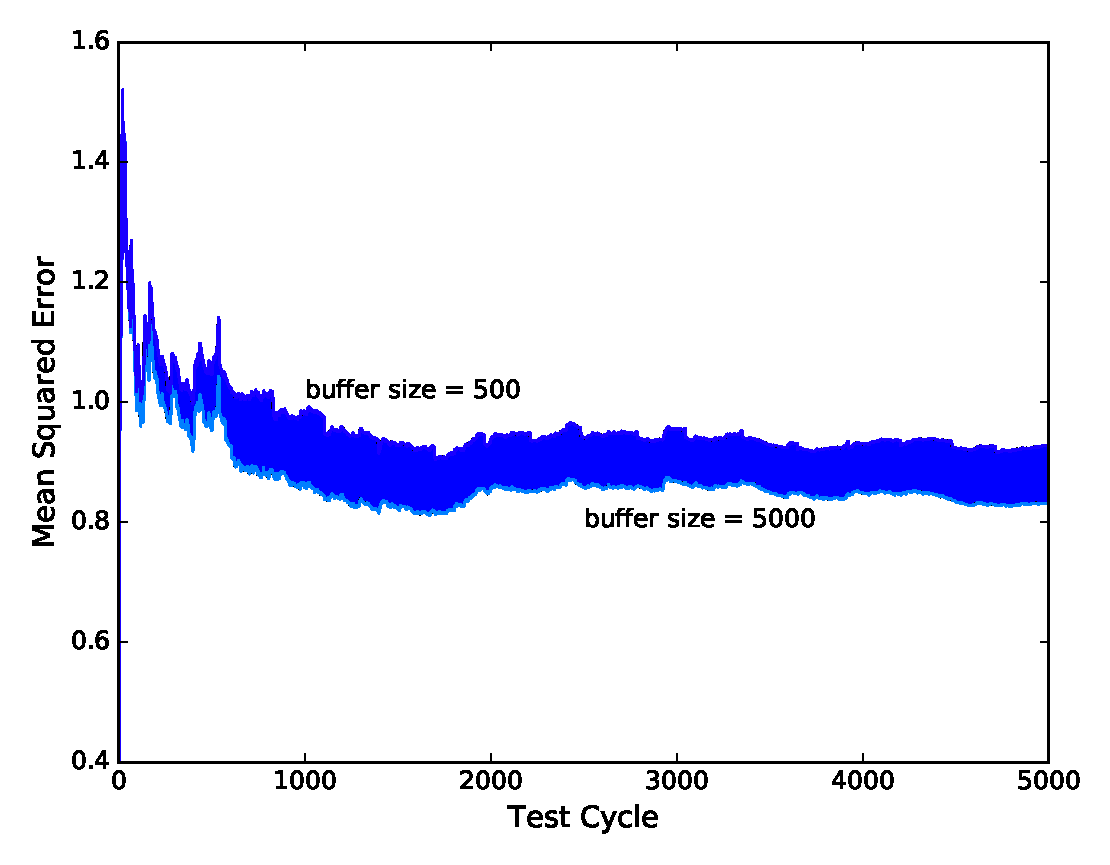
\includegraphics[width=\columnwidth]{../images/experiment-results/movie-lens-100k-buffer-size.eps}
\caption{Movie Lens 100k buffer size vs mean squared error{\color{red} make gradient or multiple lines}}
\label{fig:movie-lens-100k-buffer-size-mse}
\end{figure}

Figure \ref{fig:movie-lens-100k-buffer-size-mse} shows mean squared error for different buffer sizes for 100k MovieLens dataset. 
Smaller buffer sizes yield lower error rates, but the figure shows that the difference is small.
Specially, when considering the affect buffer size has on the running time.
Figure \ref{fig:movie-lens-100k-buffer-size-time} shows the running time on 100K MovieLens dataset using different buffer sizes. 
Increasing the buffer size from 500 to 5000 decreases the running time by a factor of 5 while the error rate is only increased slightly.
Therefore, depending on the application we can set the buffer size to bigger values in order to increase the performance of the system without affecting the quality of the final model substantially.

\begin{figure}[H]
\centering
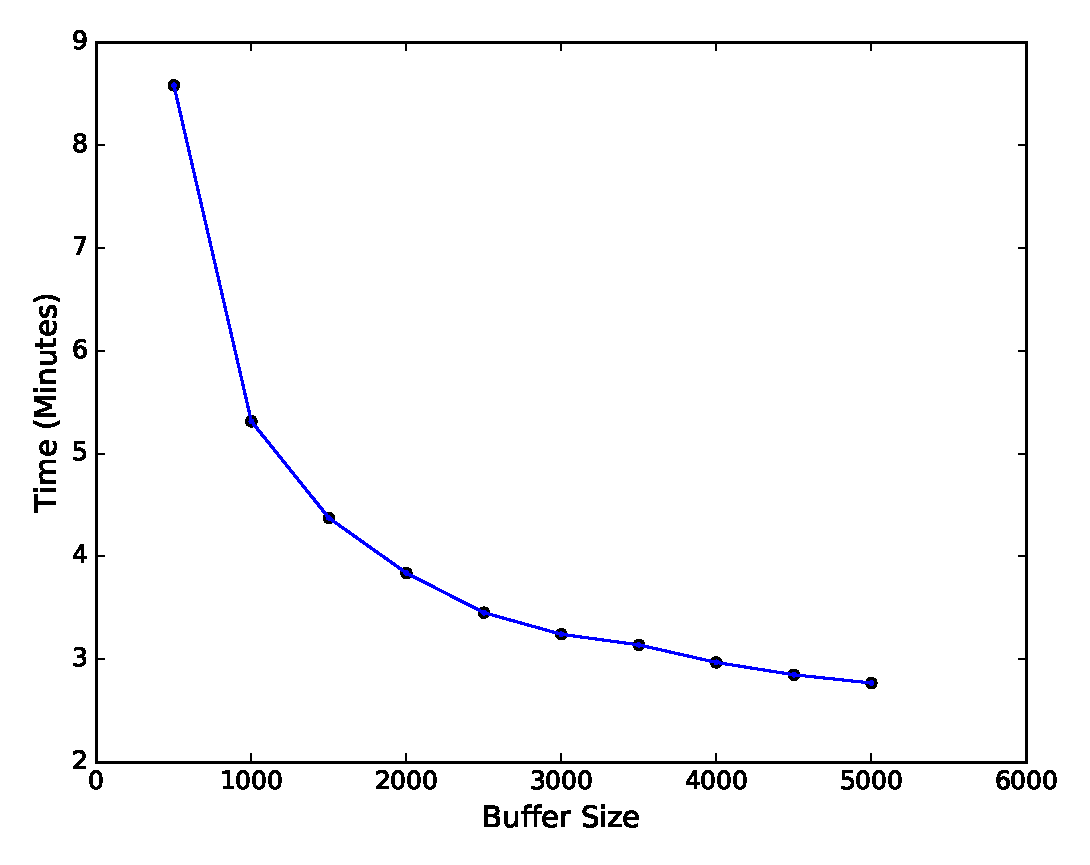
\includegraphics[width=\columnwidth]{../images/experiment-results/movie-lens-100k-buffer-time.eps}
\caption{Movie Lens 100k buffer size vs time}
\label{fig:movie-lens-100k-buffer-size-time}
\end{figure}

\textbf{Dynamic scheduling:} In production environments, the load on the system varies throughout the day. 
Therefore, a dynamic scheduling can maximizes the performance of the system, by performing more frequent updates while there are more resources available for training. 
Moreover, since training and serving can be done in parallel, we can perform training in the background and only update the weights when the training iteration is over. 

\textbf{Sampling rate}\\
In each iteration of SGD, as described in section \ref{continious-training-serving}, the data inside the buffer and a sample of the historical data is used to update the model.
In this section, we investigate the affect of the sampling rate on the model quality and running time of the system.
Figure \ref{fig:movie-lens-100k-sample-rate} shows that larger sampling rate increases the quality of the model, but similar to scheduling rate, the decrease in error rate is negligible, considering the affect it has on running time. 
 

\begin{figure}[H]
\centering
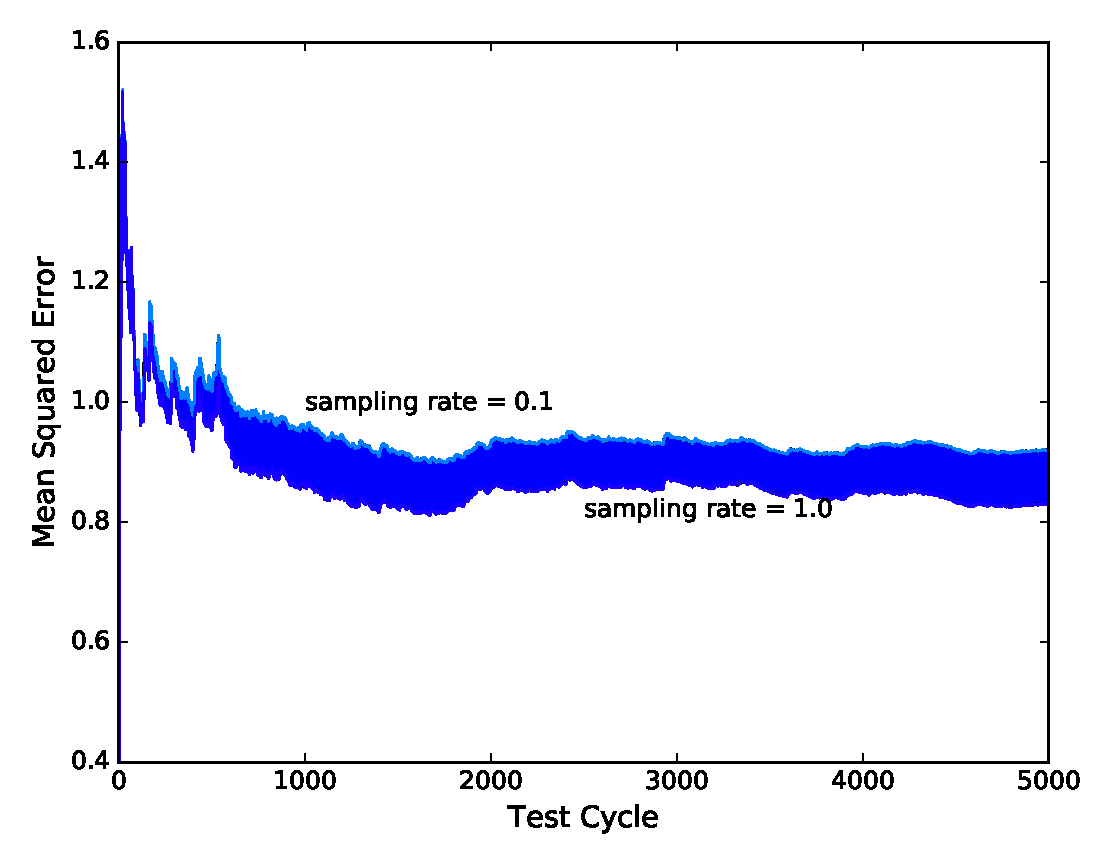
\includegraphics[width=\columnwidth]{../images/experiment-results/movie-lens-100k-sampling-rate.eps}
\caption{Movie Lens 100k sample rate vs mean squared error{\color{red} make gradient or multiple lines}}
\label{fig:movie-lens-100k-sample-rate}
\end{figure}

Figure \ref{fig:movie-lens-100k-sample-rate-time} shows that effect of increasing sampling rate on running time.
Using the entire historical data (sampling rate = 1.0) increases the running time 5 fold. 
Therefore, similar to scheduling rate, setting the sampling rate to smaller values will increase the performance substantially, while only slightly affecting the quality of the model.


\begin{figure}[H]
\centering
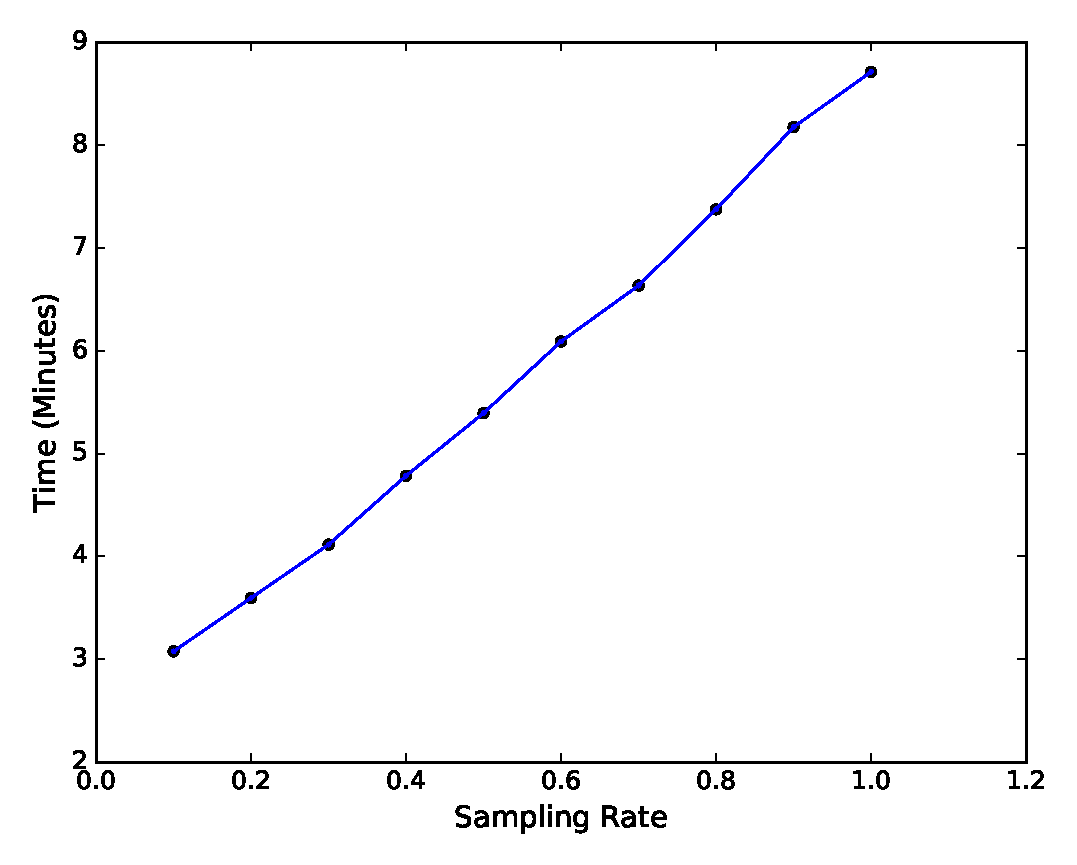
\includegraphics[width=\columnwidth]{../images/experiment-results/movie-lens-100k-sampling-time.eps}
\caption{Movie Lens 100k sampling rate vs time}
\label{fig:movie-lens-100k-sample-rate-time}
\end{figure}
%
%\subsection{Automatic tuning}
%In this section, we demonstrate the effect of automatic parameter tuning described in section \ref{sampling}, \ref{quality-monitoring}, and \ref{version-control}. 
%
%\begin{figure}[h]
%\centering
%
\includegraphics[width=\columnwidth]{../images/placeholder.jpeg}
%\caption{automatic tuning-sampling rate}
%\label{fig:tuning-sampling-rate}
%\end{figure}
%
%Figure \ref{fig:tuning-sampling-rate} shows how automatic adjustment of sampling rate could help in decreasing the overall error rate.
%
%\begin{figure}[h]
%\centering
%
\includegraphics[width=\columnwidth]{../images/placeholder.jpeg}
%\caption{automatic tuning-learning rate}
%\label{fig:tuning-learning-rate}
%\end{figure}
%
%Figure \ref{fig:tuning-learning-rate} shows how automatic adjustment of learning rate could help in decreasing the overall error rate.
%



\subsection{Methods}

In this section, we briefly describe the methods we have implemented.

\textbf{Naive} implements a simple on-line learning scenario, in which the gradient of the function at every new training item is evaluated and the weight parameters are adjusted based the gradient value. 
All the other methods also include incremental learning to constantly improve the model.

\textbf{Offline+online} is a variation of naive method, where first 10\% of the data is used for initial batch training.
The remaining data is used in an online learning fashion (on element at a time). 

\textbf{Velox} implements the proposed system by Crankshaw \cite{crankshaw2014missing}. 
In which, when the error rate on the test data passes a specified threshold, a complete retraining of the model is initiated. 
This means that the current model is replaced by a new one. 
We have implemented a variation of Velox in our experiments. 
In our implementation, retraining is initiated when a predefined number of data points have arrived at the system. 

\textbf{Continuous} is based on our proposed method. 
Once there are enough new data, the scheduler triggers a new iteration of SGD. 
The data used in this new iteration of SGD consists of the new data that arrived in the system since the last scheduled iteration plus a sample of the existing historical data.

\textbf{Baseline}: a baseline model is trained over the entire dataset and then used to calculate the test error rate. 

\subsection{Comparison Under Constrained Resources }
Both Velox and SystemX use different strategies to update the model.
To perform a fair comparison of the two, we decided to evaluate them under similar resource constraints.
We configured both Velox and SystemX frequency of training so that the total running time the given test datasets are similar.
To achieve this, we have fixed the total number of epochs (SGD iterations) for both systems.
For Velox, this value is equal to the number of retraining multiplied by number of iterations in each retraining. 
For SystemX, it is total number scheduled iterations throughout the lifetime of the system.
Therefore, SystemX schedules a new iteration every 500 items for \textit{movie-lens-100k} and xxx items for \textit{movie-lens-1M} and Velox schedules a retraining every 15,000 items for movie lens 100k and xxx items for movie lens 1M.
Figure \ref{fig:movie-lens-100k-score} and \ref{fig:movie-lens-1M-score} shows the result of this comparison.
Under similar resource constraints, SystemX perform better.
SystemX continuously makes update (batch and incremental) to the current model and builds upon the existing to model.
Whereas, Velox retrain a new model, while this new model performs better than the old model it is still losing valuable information that previous models contained.
This explains the reason SystemX performs better than Velox when under similar resource constraints.
Naive, offline+online, and baseline approaches are also included.
\todo[inline]{Add discussion of naive and offline+online}
Figure \ref{fig:movie-lens-running-time} shows the running time of the implemented methods on \textit{movie-lens-100k} and \textit{movie-lens-1M}.
\todo[inline]{Add discussion performance}

\begin{figure}[!ht]
\centering
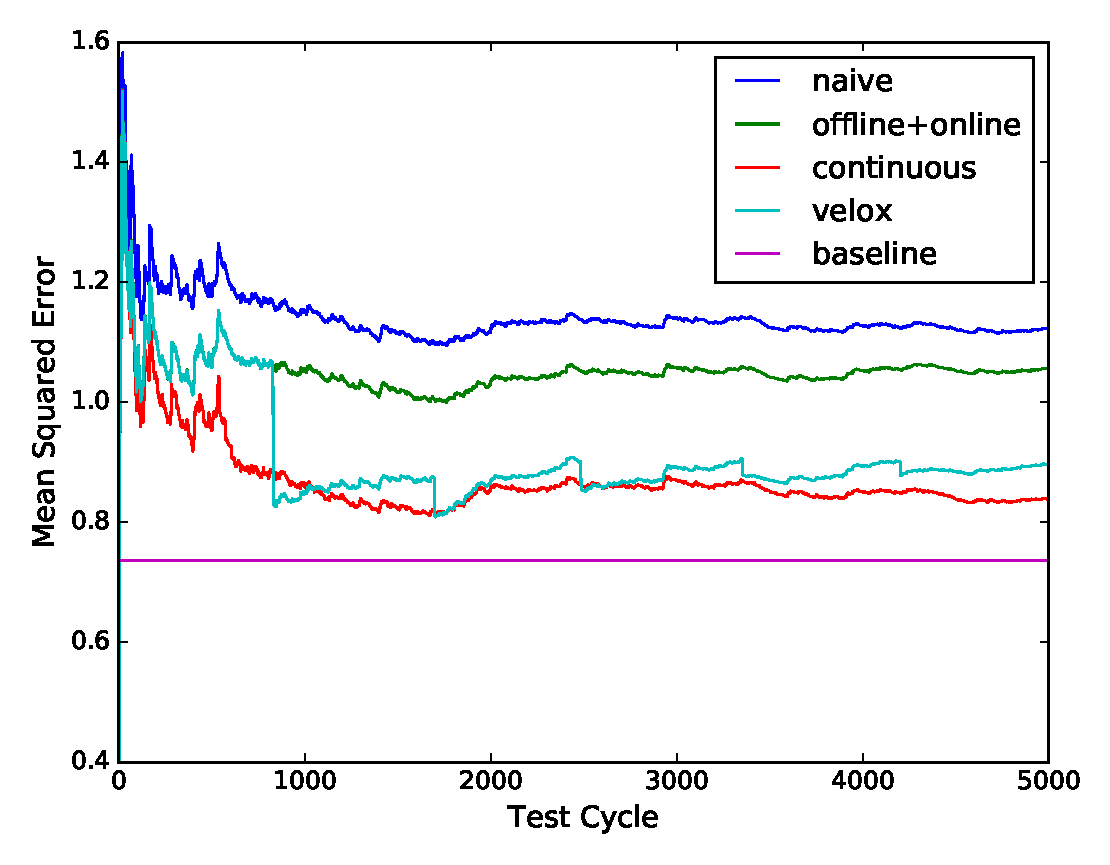
\includegraphics[width=\columnwidth]{../images/experiment-results/movie-lens-100k-quality.eps}
\caption{Mean Squared Error on Movie Lens 100k}
\label{fig:movie-lens-100k-score}
\end{figure}


\begin{figure}[!ht]
\centering
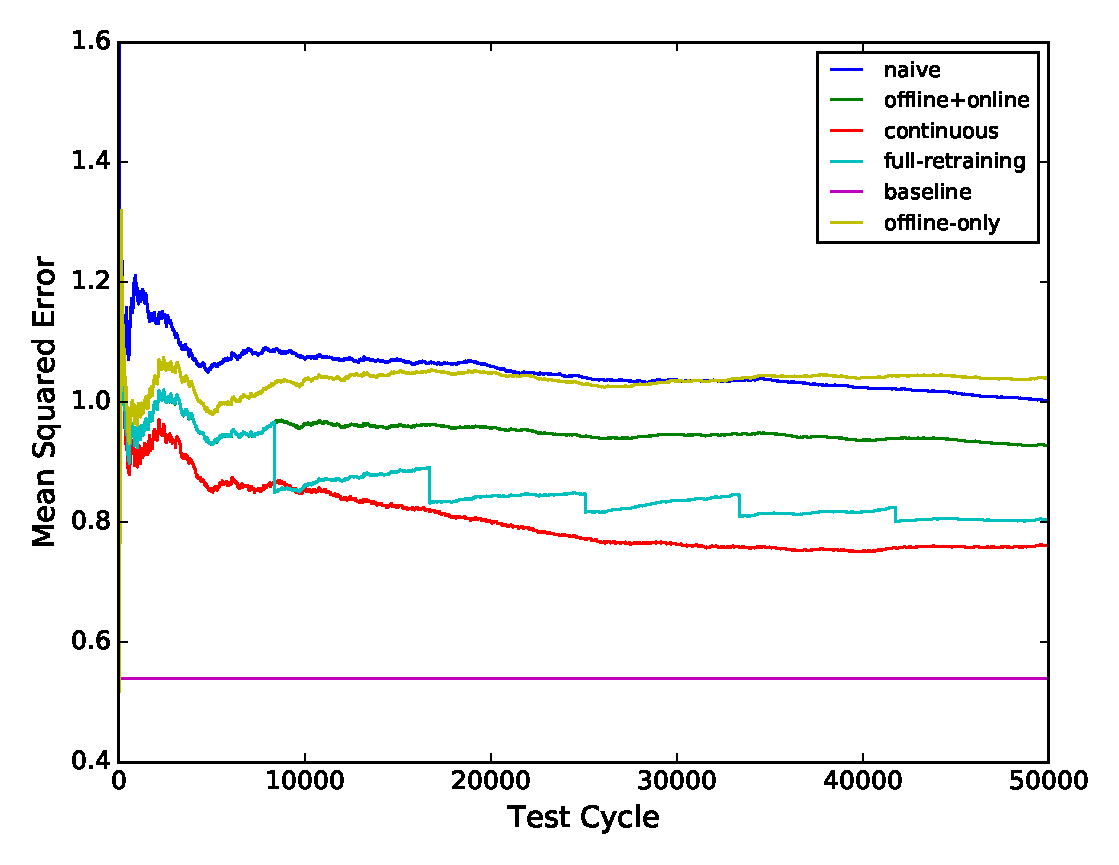
\includegraphics[width=\columnwidth]{../images/experiment-results/movie-lens-1m-quality.eps}
\caption{Mean Squared Error on Movie Lens 1M}
\label{fig:movie-lens-1M-score}
\end{figure}


\begin{figure}[!ht]
\centering
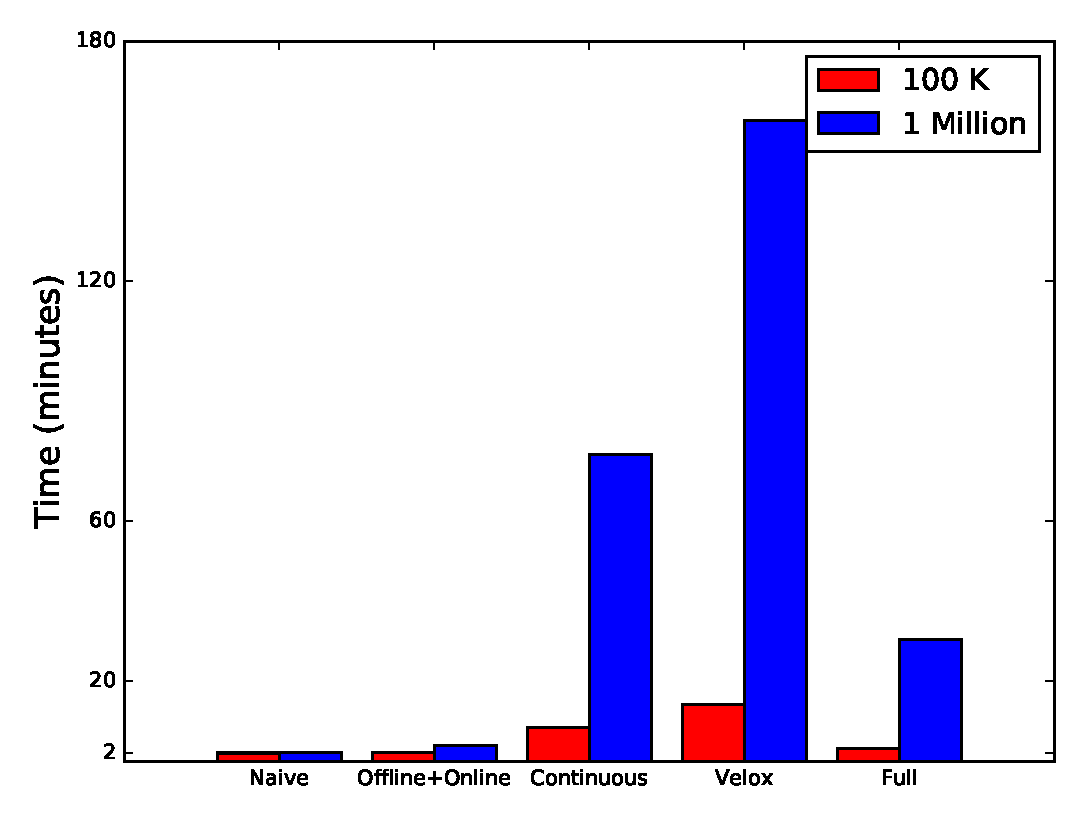
\includegraphics[width=\columnwidth]{../images/experiment-results/movie-lens-time.eps}
\caption{Running Time on Movie Lens Dataset}
\label{fig:movie-lens-running-time}
\end{figure}

\subsection{Scalability}
In this section, we compare the running time of Velox and SystemX in a distributed environment.
The actual Velox implementation is used to perform the comparisons.
We implemented SystemX on Apache Spark.

%\subsection{Quality (MSE)} 
%To measure the quality of the models, we have used an evolving test set. 
%We randomly sampled 5\% of the indices to be included in the test dataset. 
%Similar to the training data, the test set is also timestamped. 
%We start with an empty test set once the model is deployed.
%Whenever we encounter a new test item, it is added to the test set, and the mean squared error rate of the current model is calculated over this test set.
%This will indicate how the implemented models are adapting to the data being observed by the system.
%Figure \ref{fig:movie-lens-100k-score} shows the mean squared error of implemented methods on MovieLens 100k.
%Clearly, both naive and offline+online learning have lower scores than other methods.
%This is because only incremental learning is used in both of these methods.
%Velox, as described earlier retrains on the entire dataset whenever the error rate exceeds a pre-defined threshold.
%The sudden drops in error rate is where the retraining occurs.
%Our method performs consistency well and manages to reduce the error rate.
%Although initially, the error rate is slightly above Velox, continuous training manages to bridge the gap and reach the same error rate as Velox. {\color{red} This may change later if I use better system parameters}
%
%
%{\color{red}Figure \ref{fig:movie-lens-1M-score} shows the mean squared errors of the implemented methods on MovieLens 1M. 
%Similar to MovieLens 100K results, Full is performing better than all the other methods followed closely by Sample (with 40\% sampling rate) method. }
%
%\subsection{Running time} 
%
%\begin{figure}[H]
%\centering
%\includegraphics[width=\columnwidth]{../images/movie-lens-1M-time-adjusted.png}
%\caption{Running time for Movie Lens 1M}
%\label{fig:movie-lens-1M-running-time}
%\end{figure}
%
%Figure \ref{fig:movie-lens-1M-running-time} shows the running time of Sample, Full and Velox on the 1M MovieLens dataset. Depending on the sampling rate our system can be sometimes up to an order of magnitude faster that Velox. In the following section, we will investigate the effect of sampling rate on both running time and quality.

\section{Related Work} \label{related-work}
{\color{red} make it longer}

% machine learning systems for training model
Weka \cite{hall2009weka}, Apache Mahout \cite{Owen:2011:MA:2132656}, and Madlib \cite{hellerstein2012madlib} are systems that provide the necessary toolkits to train machine learning models. All of these systems provide a range of machine learning training algorithms. 
They, however, do not provide any management, before or after deployment of these models. 
Our proposed system focuses on models trainable using Stochastic Gradient Descent. 
Contrary to the systems above, it provide management of the models while in training and after deployment.
% model management systems
LongView \cite{akdere2011case}, MLBase \cite{kraska2013mlbase}, and TuPaq \cite{sparks2015tupaq} are machine learning model management systems.
They provide a range of training algorithms to create machine learning models and mechanism for model search as well as model management.
However, once models are created, they have to be deployed and used for serving manually by the users.
Our system, on the contrary, is designed for automatic deployment and continuous training.
% model serving
Tensorflow serving \cite{abadi2016tensorflow}, and others (I haven't read yet) are systems designed to manage machine learning models after they have been trained.
However, they do not handle quality control, incremental and batch updates and the user should retrain and update the models offline and deploy the new model into the system.
Our system on the other hand features a seamless process for model training, deployment, and serving. 
We provide incremental and batch updates to the model while the system is running.
% Velox
Velox \cite{crankshaw2014missing} is closest in terms of design to our system.
It provides a class of training algorithms based on the SGD optimization.
It also supports serving and incremental updates of the model after they have been deployed.
Comparing to our system however, its batch update module is out of core and offline.
Our system makes both incremental and batch updates to the models deployed while the system is running.
Our system also can make more frequent batch updates since each batch update is lightweight.

\section{Conclusions} \label{conclusion}
In conclusion, this is awesome. 
%ACKNOWLEDGMENTS are optional
\section{Acknowledgments}
\bibliographystyle{plain}
\bibliography{main}
\end{document}